\documentclass[border=10pt]{standalone}
\usepackage{pgfplots}
\pgfplotsset{compat=1.18}

\begin{document}
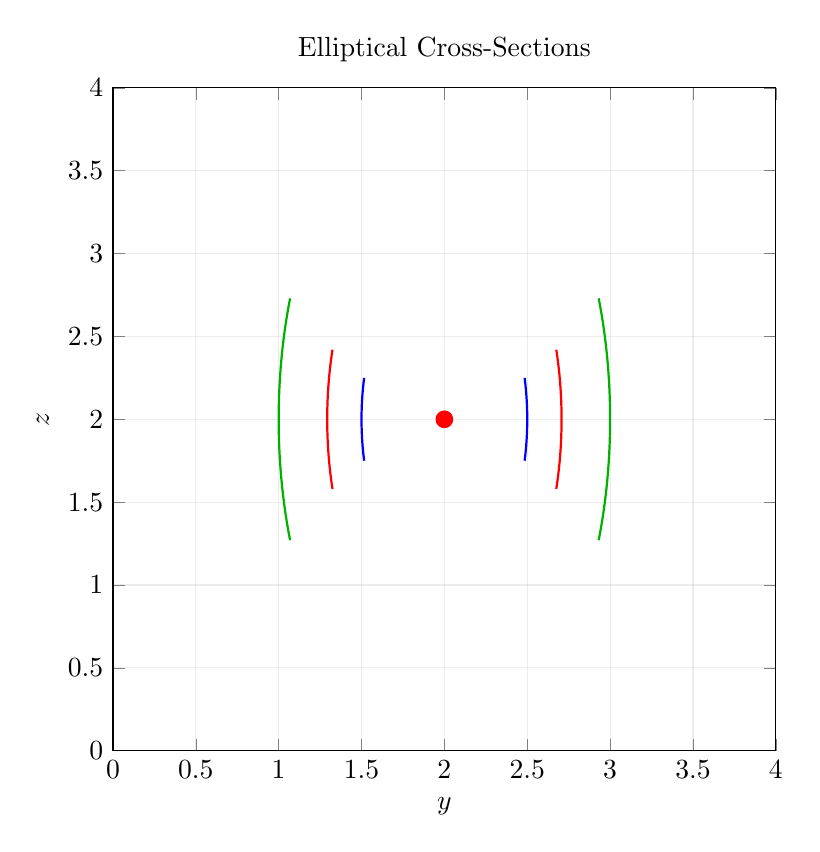
\begin{tikzpicture}
\begin{axis}[
    width=11cm,
    height=10cm,
    xlabel=$y$,
    ylabel=$z$,
    title={Elliptical Cross-Sections},
    axis equal image,
    grid=both,
    grid style={opacity=0.3},
    xmin=0, xmax=4,
    ymin=0, ymax=4,
]
% Cross-section at x=1: 4(y-2)^2 + (z-2)^2 = 1
\addplot[blue, thick, domain=1.75:2.25, samples=100] 
    ({2 + 0.5*sqrt(1 - (x-2)^2)}, x);
\addplot[blue, thick, domain=1.75:2.25, samples=100] 
    ({2 - 0.5*sqrt(1 - (x-2)^2)}, x);

% Cross-section at x=2: 4(y-2)^2 + (z-2)^2 = 2
\addplot[red, thick, domain=1.58:2.42, samples=100] 
    ({2 + 0.5*sqrt(2 - (x-2)^2)}, x);
\addplot[red, thick, domain=1.58:2.42, samples=100] 
    ({2 - 0.5*sqrt(2 - (x-2)^2)}, x);

% Cross-section at x=4: 4(y-2)^2 + (z-2)^2 = 4
\addplot[green!70!black, thick, domain=1.27:2.73, samples=100] 
    ({2 + 0.5*sqrt(4 - (x-2)^2)}, x);
\addplot[green!70!black, thick, domain=1.27:2.73, samples=100] 
    ({2 - 0.5*sqrt(4 - (x-2)^2)}, x);

% Mark center
\addplot[only marks, mark=*, mark size=3pt, red] coordinates {(2,2)};
\end{axis}
\end{tikzpicture}
\end{document}